% 3. Materials and Methods (transferred from docs/paper/paper_draft.md)
\section{Materials and Methods}
\label{sec:03_methods}

\subsection{MRI Dataset}

We used the original \texttt{.mat} release of the Cheng et al. brain tumour dataset (Figshare article 1512427, version 8, CC BY 4.0) \cite{cheng2024dataset}.

\begin{itemize}
\item \textbf{Contents:} 3,064 T1-weighted contrast-enhanced slices from 233 patients: 708 meningioma slices (82 patients), 1,426 glioma (89) and 930 pituitary (62).
\item \textbf{Integrity:} all files were verified against Figshare's published MD5 checksums and kept unmodified and read-only.
\item \textbf{Labels and patient IDs:} these were read from the original \texttt{cjdata.label} and \texttt{cjdata.PID} fields.
\item \textbf{Task:} glioma (positive) vs meningioma. Pituitary tumours were excluded from this binary task. This leaves \textbf{171 patients and 2,134 slices} (1,426 glioma, 708 meningioma), with no exact duplicate images.
\item \textbf{Preprocessing:} each slice was min–max scaled by its own intensity range (following the dataset authors' conversion script), bilinearly resized to 128×128 (15 slices are natively 256×256), and normalised with mean and standard deviation computed on the training split only. No data augmentation was used.
\end{itemize}

With slice intensities $x$, the per-slice scaling and the train-only normalisation are:

\begin{equation}
\begin{aligned}
\tilde{x} &= \frac{x - \min(x)}{\max(x) - \min(x)}, \\
\hat{x} &= \frac{\mathrm{resize}_{128\times128}(\tilde{x}) - \mu_{\mathrm{train}}}{\sigma_{\mathrm{train}}}
\end{aligned}
\label{eq:1}
\end{equation}

\textbf{Possible site-related confounding.} Patient IDs occur in two formats: \texttt{MR}-prefixed IDs and purely numeric IDs. All 67 \texttt{MR}-prefixed patients are gliomas; the 104 numeric-ID patients comprise 22 gliomas and 82 meningiomas. The dataset documentation reports acquisition at two hospitals but does not say what the ID formats mean. The association may therefore reflect site or scanner differences, but this is not established. Absolute classification performance must be interpreted cautiously. The confound affects all compared models identically.

\subsection{Leakage-Safe Patient-Level Evaluation}

\textbf{Conservative grouping of possibly related examinations.} Some \texttt{MR}-prefixed IDs share a base number and differ only by a letter suffix (for example \texttt{MR040240}, \texttt{MR040240B}, \texttt{MR040240C}, \texttt{MR040240D}). Whether these are the same person is unknown. As a conservative leakage-prevention assumption, we assigned a \texttt{patient\_link\_key} (regular expression \texttt{\textasciicircum{}(?P<base>MR\textbackslash{}d\{6\})[A-Z]?\$}) that groups 42 IDs into 18 families. The published \texttt{patient\_id} values were not changed.

\textbf{Fixed split (initial experiments).} A deterministic, class-stratified group split (seed 0) assigned entire linked groups to one partition:

\begin{itemize}
\item train: 124 patients, 1,506 slices;
\item validation: 26 patients, 326 slices;
\item test: 21 patients, 302 slices.
\end{itemize}

There was no patient or link-key overlap between partitions.

\textbf{Leakage-safe cross-validation using the official Figshare outer test folds (main experiment).} The dataset provides official five-fold indices (\texttt{cvind.mat}), which map cleanly to the published patient IDs. However, 16 of the 18 link families span different official folds. For outer fold \emph{k}:

\begin{itemize}
\item \textbf{Test:} the official fold \emph{k}, \textbf{unchanged}.
\item \textbf{Validation:} the next official fold, cyclically (1→2, 2→3, 3→4, 4→5, 5→1), minus any patient whose link key occurs in the test set.
\item \textbf{Training:} the remaining three folds, minus any patient whose link key occurs in the test set or in the cleaned validation set.
\end{itemize}

No patient was moved between folds or replaced. Official fold values were not altered. Between 11 and 19 linked patients were excluded from training and validation per outer fold; all of them were \texttt{MR}-prefixed gliomas. The resulting partitions have zero \texttt{patient\_id} and zero \texttt{patient\_link\_key} overlap in every fold, and \textbf{every one of the 171 patients is in exactly one outer test fold}.

This is therefore \emph{not} an exact reproduction of the dataset authors' five-fold protocol. It preserves their test folds but applies an additional exclusion rule to training and validation. The training \texttt{pos\_weight} (negatives/positives) and the normalisation statistics were recomputed per fold from the cleaned training set only, giving \texttt{pos\_weight} values of 0.679, 0.663, 0.779, 0.798 and 0.597 for folds 1–5.

\begin{figure*}[!t]
\centering
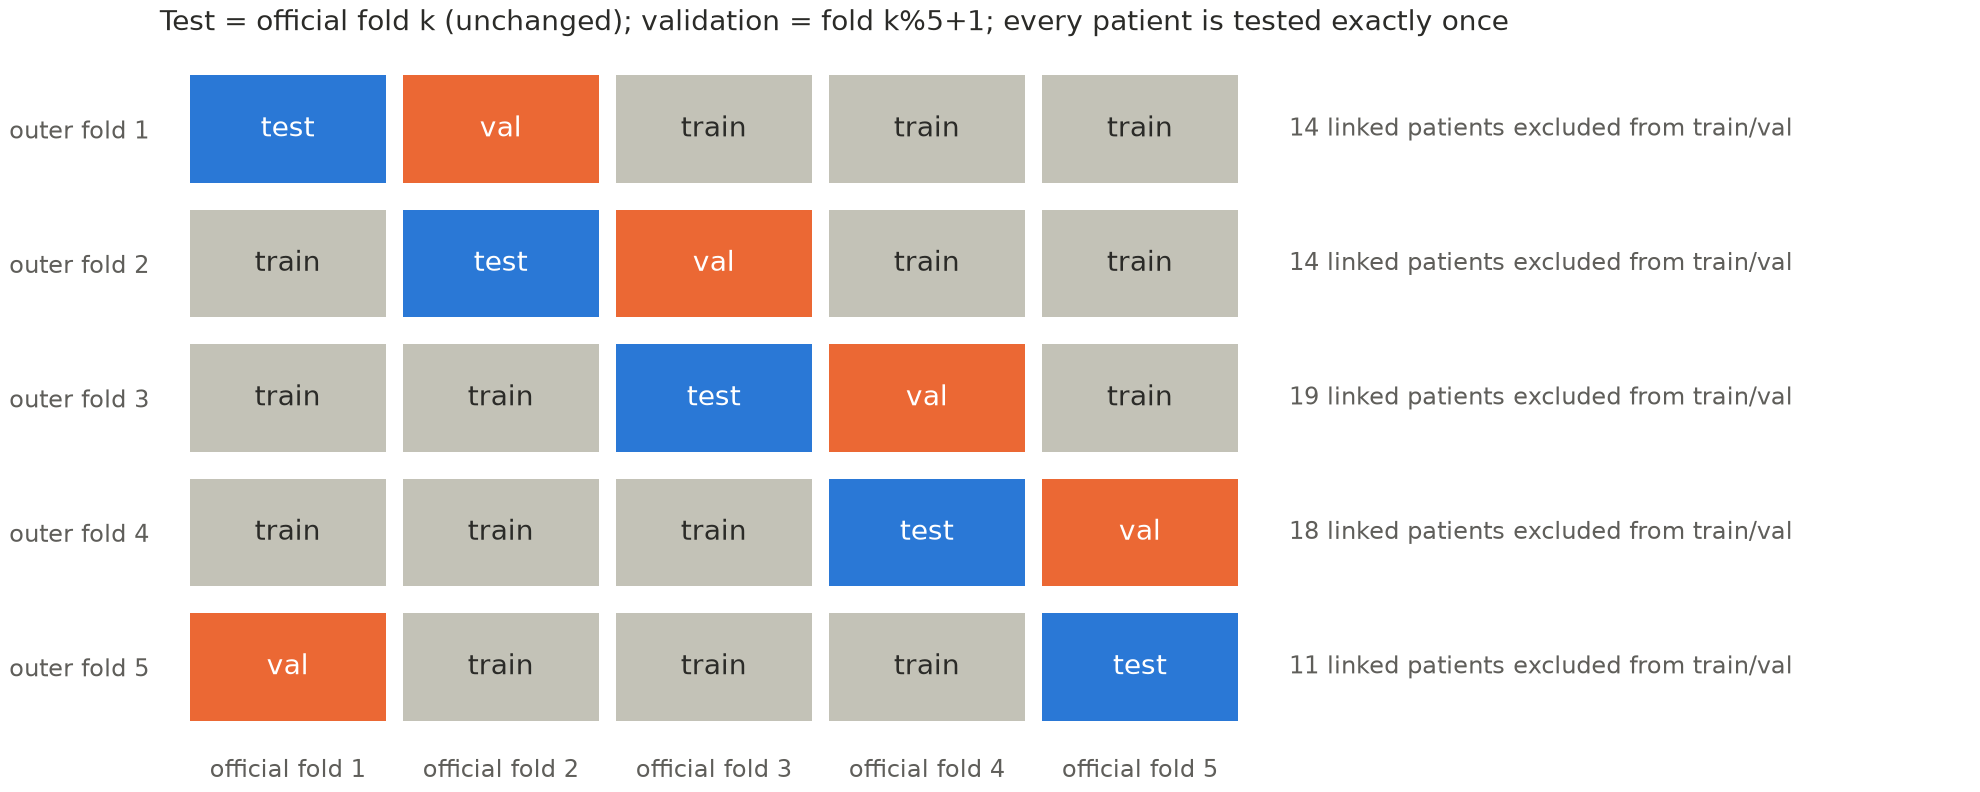
\includegraphics[width=\textwidth]{figures/fig_cv_design.png}
\caption{Leakage-safe cross-validation using the official Figshare outer test folds. For outer fold k, the official fold k is the unchanged test set and fold k\%5+1 is the validation set; linked relatives of test and validation patients are excluded from validation/training (numbers per fold). Every patient is tested exactly once, which yields the pooled out-of-fold (OOF) predictions.}
\label{fig:fig_cv_design}
\end{figure*}

\subsection{Drosophila Connectome Construction}

\textbf{Source and extraction.} Connectivity was obtained from MaleCNS v1.0 \cite{malecns} through neuPrint \cite{neuprint} (\texttt{male-cns:v1.0}, neuprint-python 0.6.3, database uuid \texttt{4b2087c0…}). For a selected set of neurons we retrieved all directed connections among them.

\begin{itemize}
\item \textbf{Edges and weights:} an edge \emph{i→j} carries the total synapse count from presynaptic neuron \emph{i} to postsynaptic neuron \emph{j}.
\item \textbf{Validation:} edge lists were checked for missing values, non-positive weights and duplicates.
\item \textbf{Isolated neurons:} kept as nodes.
\item \textbf{Self-loops:} removed before use.
\item \textbf{Provenance:} all downloads are recorded with checksums.
\end{itemize}

\textbf{Engineering graph (EB).} Before selecting a visual graph, we validated the pipeline on a \emph{generic} graph: the 128 neurons with the most synapses in the ellipsoid body (EB), a navigation-related central-complex region that is not part of the visual system. With all connections kept, this graph had a density of 0.79. Before any MRI training we pre-declared a sparser variant keeping only edges with at least 20 synapses (w20). It has 3,047 edges, density 0.187, reciprocity 0.52, clustering 0.50 and one strongly connected component. The EB graph is reported only as an initial topology experiment and is never labelled as visual.

\subsection{Visual-System Graph Selection}

\textbf{Choice of strategy.} We compared three candidate strategies on biological and graph criteria only, without using MRI data:

\begin{itemize}
\item (A) the top-128 neurons by synapse count in the medulla ME(R);
\item (B) an annotation-defined local retinotopic patch;
\item (C) the top-128 right-side visual projection neurons.
\end{itemize}

Strategy B was chosen. It represents a canonical, repeated circuit, is defined only by verified annotations, and is naturally sparse.

\textbf{Selection rule for strategy B.}

\begin{itemize}
\item \textbf{Candidates:} neurons of 11 columnar cell types of the ON/OFF motion-pathway input stage (L1, L2, L3, Mi1, Mi4, Mi9, C3, Tm1, Tm2, Tm4, Tm9) that have synapses in ME(R) and an assigned retinotopic column (\texttt{assignedOlHex1/2}).
\item \textbf{Central column:} the median (hex1, hex2) over the 817 columns containing all 11 types, which is (18, 20).
\item \textbf{Ordering:} neurons were ordered by hexagonal distance from the central column, with neighbour offsets verified on L1 soma positions, then by column coordinates, fixed type order and bodyId. The first 128 were kept.
\end{itemize}

The resulting patch spans 12 columns: the central column and its first ring are complete, and the second ring is partially filled. It contains 12 neurons of each of L1, L2, L3, Mi1, Mi4, Mi9 and C3, and 11 of each of Tm1, Tm2, Tm4 and Tm9.

\textbf{Properties of the primary graph} (all edges retained, weight ≥ 1):

\begin{itemize}
\item 989 directed edges, density 0.061;
\item mean in/out-degree 7.7, maximum in-degree 38 and out-degree 20;
\item reciprocity 0.51, clustering 0.38;
\item 12 strongly connected components, the largest with 117 nodes.
\end{itemize}

\textbf{Biological plausibility.} The strongest type-to-type connections reproduce known pathways: L2→Tm2/Tm1/Tm4, L1→Mi1, L3→Mi9, Mi4→Mi9 and C3→L2. The small strongly connected components have a biological explanation: seven L3 cells receive their input from photoreceptors, and three Tm9 cells project to T5, neither of which is included.

\textbf{What is not included.} T4/T5 and Tm3 have no column assignment in MaleCNS. They were not included, and no column was inferred for them. The graph is therefore a local input-stage circuit, not a complete motion detector. A variant keeping only edges of at least 5 synapses (w≥5, 411 edges) was defined as a sensitivity analysis only and is not part of the results reported here.

\subsection{Control Graphs}

For each biological graph, control graphs were generated from five seeds (0–4). Each has the same 128 nodes and \textbf{exactly the same number of directed edges}, with no self-loops. Training seed \emph{s} is paired with control-graph seed \emph{s}.

\begin{itemize}
\item \textbf{Degree-preserving rewired (primary null model):}
\begin{itemize}
\item \textbf{Construction:} directed double-edge swaps, 10 attempted swaps per edge (Eq. 2). A swap is rejected if it would create a self-loop or a duplicate edge.
\end{itemize}
\end{itemize}

\begin{equation}
\begin{aligned}
&(a \rightarrow b,\; c \rightarrow d) \;\longmapsto\; (a \rightarrow d,\; c \rightarrow b), \\
&a \neq d,\; c \neq b,\; (a \rightarrow d),(c \rightarrow b) \notin \mathcal{E}
\end{aligned}
\label{eq:2}
\end{equation}

\begin{itemize}
\begin{itemize}
\item \textbf{What it preserves:} every node's exact in- and out-degree.
\item \textbf{What it destroys:} the biological partner identities. On the visual graph, reciprocity drops from 0.51 to 0.08 and clustering from 0.38 to 0.10 (means over seeds), and 13\% of edges coincide with biological edges, near the chance level for the given degree sequence.
\end{itemize}
\item \textbf{Erdős–Rényi (ER):} directed G(n, m); edges uniformly at random among all ordered pairs.
\item \textbf{Watts–Strogatz-type (WS):} a directed variant defined in the project. It starts from a ring lattice with the exact edge count and rewires each edge's target with probability 0.1. It has high reciprocity (0.80) and clustering (0.48) but nearly uniform degrees.
\item \textbf{Barabási–Albert-type (BA):} a directed variant defined in the project, built from undirected preferential attachment with random edge directions and trimmed to the exact edge count. It produces hubs and has zero reciprocity.
\end{itemize}

The directed WS and BA constructions are project-specific documented definitions, not universal standards. Their construction rules are frozen and guarded by golden-hash regression tests.

\begin{table*}[!t]
\settablenumber{II}
\centering
\footnotesize
\caption{Visual graph and control graph properties (128 nodes and 989 edges each; controls: mean over seeds 0–4).}
\label{tab:II}
\begin{tabular}{lcccccc}
\toprule
\textbf{Graph} & \textbf{Density} & \textbf{Max in / out degree} & \textbf{Reciprocity} & \textbf{Clustering} & \textbf{SCCs} & \textbf{Overlap with biological edges} \\
\midrule
Visual Drosophila (w≥1) & 0.061 & 38 / 20 & 0.510 & 0.381 & 12 (largest 117) & 1.000 \\
Degree-preserving rewired & 0.061 & 38 / 20 & 0.084 & 0.097 & 11.2 & 0.130 \\
ER & 0.061 & 14.4 / 15.6 & 0.057 & 0.062 & 1.2 & 0.057 \\
WS (directed variant) & 0.061 & 11.2 / 8.0 & 0.795 & 0.479 & 1.0 & 0.065 \\
BA (directed variant) & 0.061 & 29.2 / 28.6 & 0.000 & 0.102 & 1.0 & 0.056 \\
\emph{Reference:} EB w20 (Phase 8) & 0.187 & 53 / 71 & 0.519 & 0.496 & 1 & n/a (3,047 edges) \\
\bottomrule
\end{tabular}
\end{table*}

\begin{figure*}[!t]
\centering
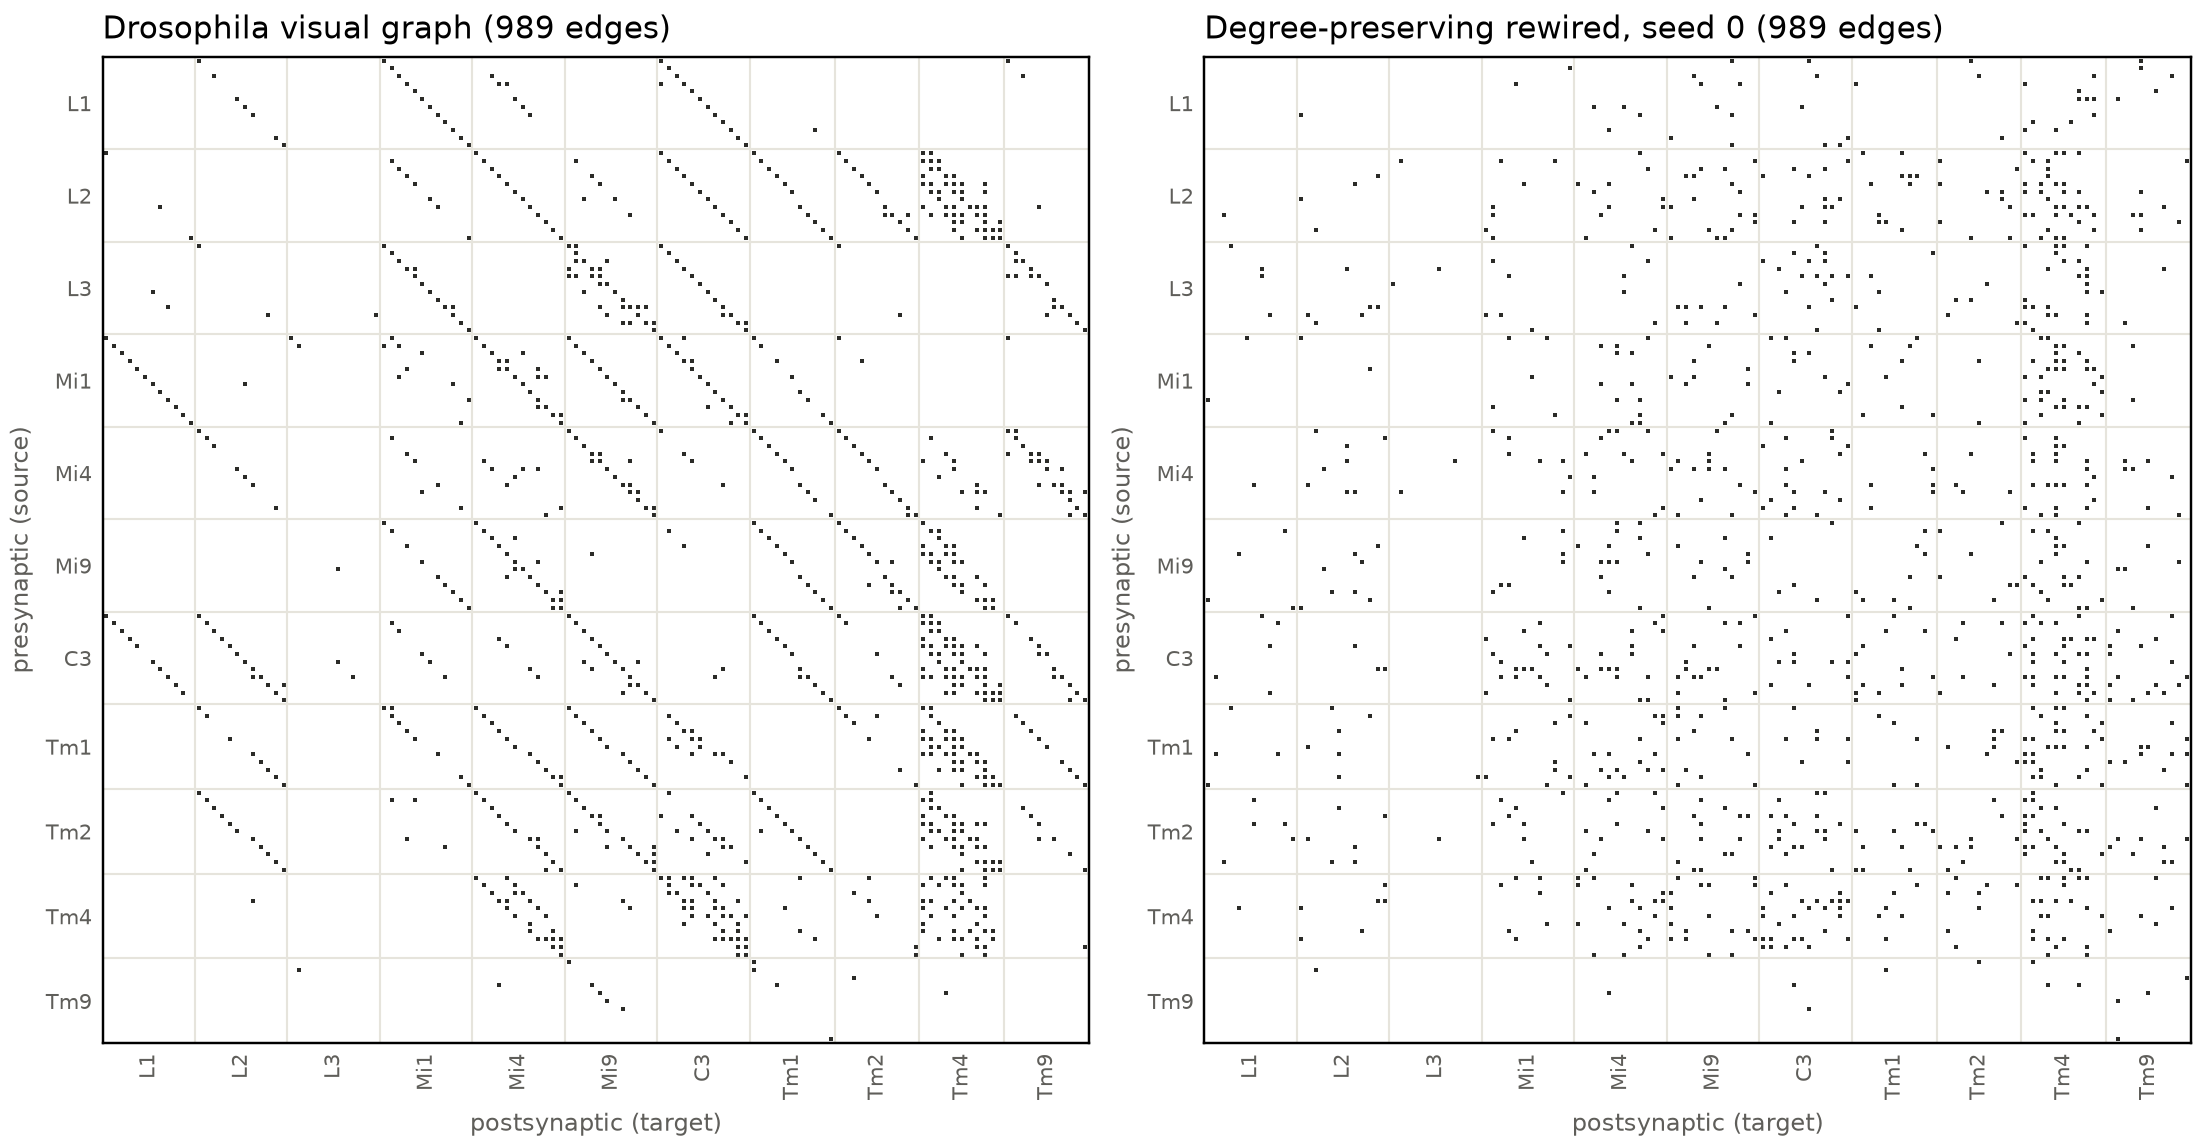
\includegraphics[width=\textwidth]{figures/fig_adjacency.png}
\caption{Adjacency matrices of the Drosophila visual graph (left) and its degree-preserving rewired control, seed 0 (right). Rows are presynaptic and columns postsynaptic neurons, ordered by cell type and then by retinotopic column. Row and column sums (in- and out-degrees) are identical in both panels; the rewired graph loses the biological block structure. Drawn directly from the frozen edge files.}
\label{fig:fig_adjacency}
\end{figure*}

\subsection{Neural Network Architectures}

All models share one small CNN encoder (Fig. 3):

\begin{itemize}
\item 1×128×128 input;
\item Conv3×3(1→16)–ReLU–MaxPool;
\item Conv3×3(16→32)–ReLU–MaxPool;
\item Conv3×3(32→128)–ReLU;
\item global average pooling, giving a 128-dimensional feature vector.
\end{itemize}

It has no batch normalisation, dropout, pretraining or augmentation.

\begin{figure*}[!t]
\centering
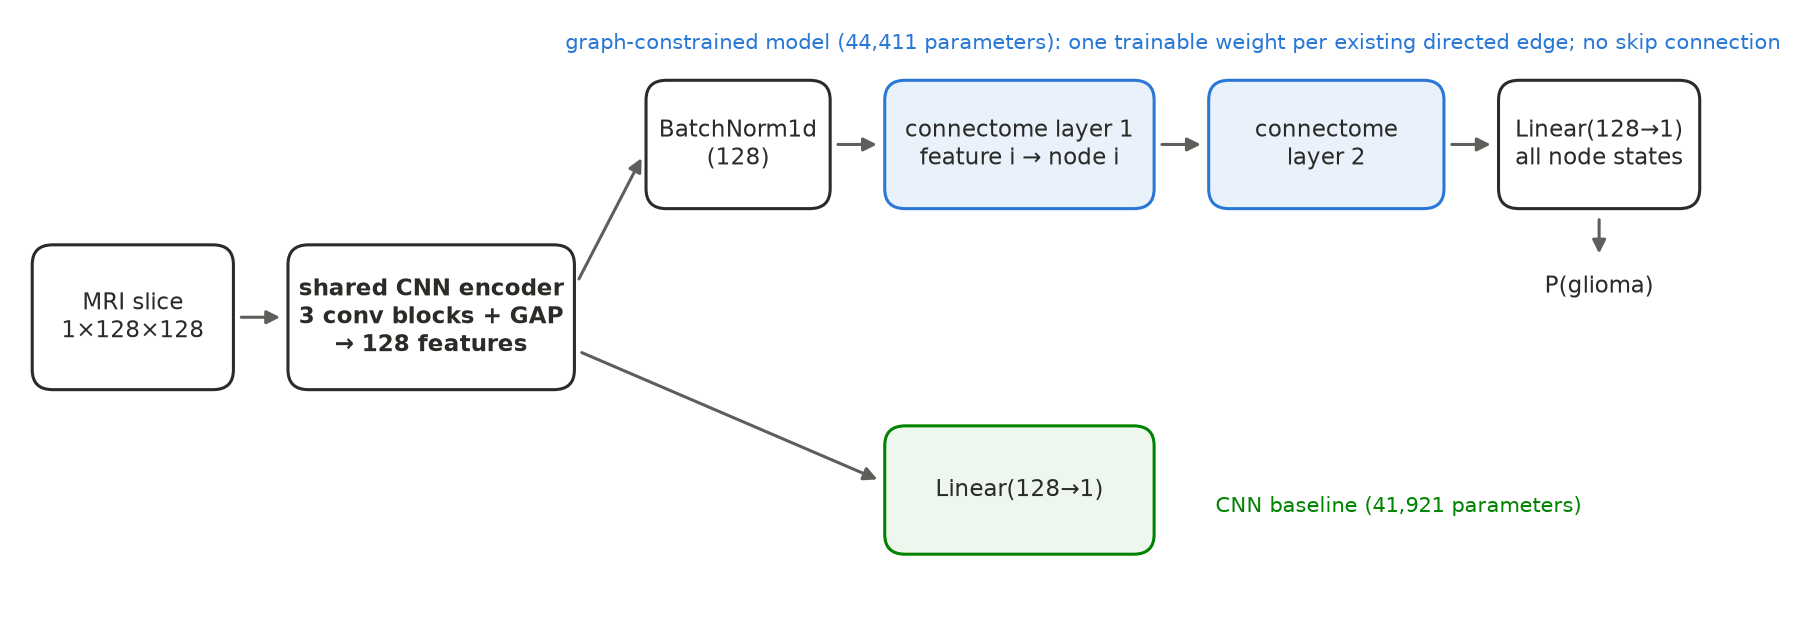
\includegraphics[width=\textwidth]{figures/fig_pipeline.png}
\caption{Model overview. A shared CNN encoder maps a 1×128×128 slice to 128 features. The CNN baseline (bottom) applies a linear classifier directly. The graph-constrained model (top) batch-normalises the features, assigns feature i to graph node i, propagates them through two connectome-constrained layers (one trainable weight per existing directed edge, no skip path) and reads all 128 final node states with a linear classifier.}
\label{fig:fig_pipeline}
\end{figure*}

\textbf{CNN baseline.} The 128 features feed a Linear(128→1) layer. It has 41,921 parameters.

\textbf{Graph-constrained model.} The 128 features are batch-normalised (BatchNorm1d), and feature \emph{i} initialises the scalar state of graph node \emph{i}. Two propagation layers then update the node states (Eqs. 3–6 below):

\begin{itemize}
\item \textbf{Signal direction:} signals flow only from presynaptic to postsynaptic nodes.
\item \textbf{Edge weights:} there is exactly one trainable weight per existing edge, with fan-in initialisation. Non-existent edges have no parameter, which is equivalent to $W \odot A$ for a binary adjacency mask $A$. Synapse counts define which edges exist, not their initial strength.
\item \textbf{Output:} all 128 final node states feed a Linear(128→1) classifier.
\item \textbf{No bypass:} there is no skip connection from encoder to classifier, so all information reaching the prediction passes through the graph.
\end{itemize}

Formally, let $\phi$ denote the convolutional encoder with global average pooling, $\mathcal{E}$ the directed edge set and $A$ its binary adjacency matrix ($A_{ij}=1$ if $(i\rightarrow j)\in\mathcal{E}$). The graph model computes

\begin{equation}
\mathbf{f} = \phi(\hat{x}) \in \mathbb{R}^{128}, \qquad \mathbf{h}^{(0)} = \mathrm{BN}(\mathbf{f})
\label{eq:3}
\end{equation}

\begin{equation}
h^{(\ell)}_j = \mathrm{ReLU}\left( \sum_{i:\,(i\rightarrow j)\in\mathcal{E}} w^{(\ell)}_{ij}\, h^{(\ell-1)}_i + b^{(\ell)}_j \right), \qquad \ell = 1, 2
\label{eq:4}
\end{equation}

which is equivalent to the masked dense form

\begin{equation}
\mathbf{h}^{(\ell)} = \mathrm{ReLU}\left( \left(W^{(\ell)} \odot A\right)^{\top} \mathbf{h}^{(\ell-1)} + \mathbf{b}^{(\ell)} \right)
\label{eq:5}
\end{equation}

in which only the $|\mathcal{E}|$ entries of $W^{(\ell)}$ with $A_{ij}=1$ exist as parameters. The weights and output are

\begin{equation}
\begin{aligned}
&w^{(\ell)}_{ij} \sim \mathcal{U}\left(-\frac{1}{\sqrt{k^{\mathrm{in}}_j}},\, \frac{1}{\sqrt{k^{\mathrm{in}}_j}}\right), \quad b^{(\ell)}_j = 0, \\
&z = \mathbf{v}^{\top}\mathbf{h}^{(2)} + c, \quad p = \sigma(z)
\end{aligned}
\label{eq:6}
\end{equation}

where $k^{\mathrm{in}}_j$ is the in-degree of node $j$ (at least 1). The CNN baseline uses $z = \mathbf{v}^{\top}\mathbf{f} + c$.

The visual-graph models have 44,411 parameters: encoder 41,792, BatchNorm 256, graph block 2×(989+128), classifier 129. The EB-graph models have 48,527. Graph models with equal edge counts have identical parameter counts.

\textbf{Development note.} A first specification with mean pooling over nodes followed by Linear(1→1) collapsed to constant predictions (validation AUC exactly 0.5). The image-dependent signal shrank through the sparse layers and was averaged into a single scalar. This was an architectural bottleneck, not a biological result. It was corrected (BatchNorm plus a full readout) before any controlled comparison, the corrected architecture was frozen, and it is identical for all graphs.

\textbf{Tests.} Unit tests verify that:

\begin{itemize}
\item forbidden edges contribute nothing and receive exactly zero gradient;
\item allowed edges receive gradients;
\item edge direction is respected;
\item removing an edge changes the output;
\item silencing the graph makes the output independent of the input image.
\end{itemize}

\subsection{Training Protocol}

All settings were frozen before the first comparison and are identical across models:

\begin{itemize}
\item \textbf{Loss:} binary cross-entropy with logits and \texttt{pos\_weight} = \#meningioma / \#glioma, computed on the training split only.
\item \textbf{Optimiser:} Adam (learning rate 10⁻³, weight decay 10⁻⁴), batch size 32, at most 30 epochs.
\item \textbf{Model selection:} the checkpoint with the best validation slice-level ROC AUC (ties to the earlier epoch), with early stopping after 7 epochs without improvement.
\item \textbf{Validation sanity gate:} it checks only for technical degeneration (non-finite values, constant predictions, dead graph output) and has no performance threshold. The test data were loaded only after training, checkpoint selection and this gate.
\item \textbf{Failed runs:} runs failing the gate would have been recorded and not replaced; none occurred.
\item \textbf{Determinism:} seeds were fixed for Python, NumPy and PyTorch. Training was done on CPU. Re-running a configuration reproduced its predictions bit for bit.
\end{itemize}

For a mini-batch of $B$ slices with labels $y_n \in \{0,1\}$ (1 = glioma), the loss is

\begin{equation}
\begin{aligned}
\mathcal{L} &= -\frac{1}{B}\sum_{n=1}^{B}\left[\pi\, y_n \log\sigma(z_n) + (1-y_n)\log\left(1-\sigma(z_n)\right)\right], \\
\pi &= \frac{N^{\mathrm{train}}_{\mathrm{meningioma}}}{N^{\mathrm{train}}_{\mathrm{glioma}}}
\end{aligned}
\label{eq:7}
\end{equation}

\subsection{Evaluation Metrics}

The primary metric is \textbf{patient-level ROC AUC}: a patient's probability is the mean of their slice probabilities, and hard labels are never averaged. Secondary metrics are slice-level ROC AUC, balanced accuracy, sensitivity (glioma), specificity (meningioma), F1, precision, recall and confusion matrices. The threshold-dependent metrics use a fixed threshold of 0.5 that was never tuned.

For patient $k$ with slice set $S_k$,

\begin{equation}
P_k = \frac{1}{|S_k|}\sum_{s\in S_k} p_s, \qquad \hat{y}_k = \mathbf{1}\left[P_k \geq 0.5\right]
\label{eq:8}
\end{equation}

\begin{equation}
\begin{aligned}
\mathrm{Sens} &= \frac{TP}{TP+FN}, \quad \mathrm{Spec} = \frac{TN}{TN+FP}, \\
\mathrm{BalAcc} &= \frac{\mathrm{Sens}+\mathrm{Spec}}{2}
\end{aligned}
\label{eq:9}
\end{equation}

In cross-validation we report:

\begin{itemize}
\item \textbf{Run level:} all 25 fold×seed runs per model.
\item \textbf{Fold level:} seeds averaged within each fold, then mean ± SD across the 5 folds. This is the main robustness summary.
\item \textbf{Pooled out-of-fold (OOF):} for each model and seed, the five outer-test folds are concatenated so that every patient is predicted exactly once, and metrics are computed on this pooled set. We report mean ± SD across seeds.
\end{itemize}

Paired comparisons match runs strictly by outer fold and seed. For outer fold $f$ and seed $s$:

\begin{equation}
\begin{aligned}
\Delta_{f,s} &= \mathrm{AUC}^{\mathrm{Drosophila}}_{f,s} - \mathrm{AUC}^{\mathrm{rewired}}_{f,s}, \\
\bar{\Delta}_f &= \frac{1}{5}\sum_{s=0}^{4}\Delta_{f,s}
\end{aligned}
\label{eq:10}
\end{equation}

We report the mean ± SD of the 25 values $\Delta_{f,s}$ and of the 5 fold-level values $\bar{\Delta}_f$. All statistics are descriptive; no significance tests were performed.
